\documentclass[a4paper,12pt]{article}
\usepackage{graphicx}
\usepackage[left=2.5cm, right=2.5cm, top=3cm, bottom=3cm]{geometry}
\usepackage{amsmath, amsthm, amssymb}
\usepackage[left=2.5cm, right=2.5cm, top=3cm, bottom=3cm]{geometry}
\usepackage[hidelinks]{hyperref}
\usepackage[spanish]{babel}
\usepackage{cite}
\usepackage{color}
\usepackage{url}

\begin{document}
\title{\Huge \textbf{Moogle!}}
\author{Diego Manuel Viera Martínez}
\date{julio , 2023}
\maketitle
\begin{center}
    
\includegraphics[scale=0.7]{Pictures/matcom.jpg}\label{fig:logo}
\end{center}

\begin{center}
   \Huge Primer proyecto de programación
\end{center}

\newpage
\section{Introducción}\label{sec:intro}

Bienvenidos a MOOGLE! el buscador más rápido hasta la fecha. Con esta poderosa herramineta podrás hacer búsquedas sobre tus documentos
de manera rápida y eficiente, con funcionalidades extra como acceder al documento o obtener información previa, con un diseño minimalista y simple 
para un fácil uso de este. A continuación se explicará con mayor detalle el poder de este buscador.

\section{¿Cómo empezar a usarlo?}\label{sec:start}

\subsection{Pasos para obtener y empezar a usar MOOGLE!}

\begin{enumerate}
    \item Descargue el .zip del proyecto en este repositorio de github \url{https://github.com/DiegoViera1511/Proyecto-I-Moogle}
    \item Descomprimir el archivo .zip
    \item Añadir en la carpeta \texttt{Content} su base de datos, en la cual se realizarán las búsquedas.
    \item Ahora ejecute en su terminal el archivo \texttt{proyecto.sh} y seleccione la opción \texttt{run}
    \item  Listo, ya puede disfrutar de MOOGLE!
\end{enumerate}
 
Puede ejecutar el proyecto manualmente abriendo la terminal de su PC y ubíquese en la carpeta que contiene al proyecto, luego de esto ejecutar el comando \texttt{make dev}.
En el caso de una PC Windows deberá ejecutar el comando dotnet \texttt{watch run --project MoogleServer}

\subsection{¿Cómo hacer una búsqueda?}
\begin{center}
    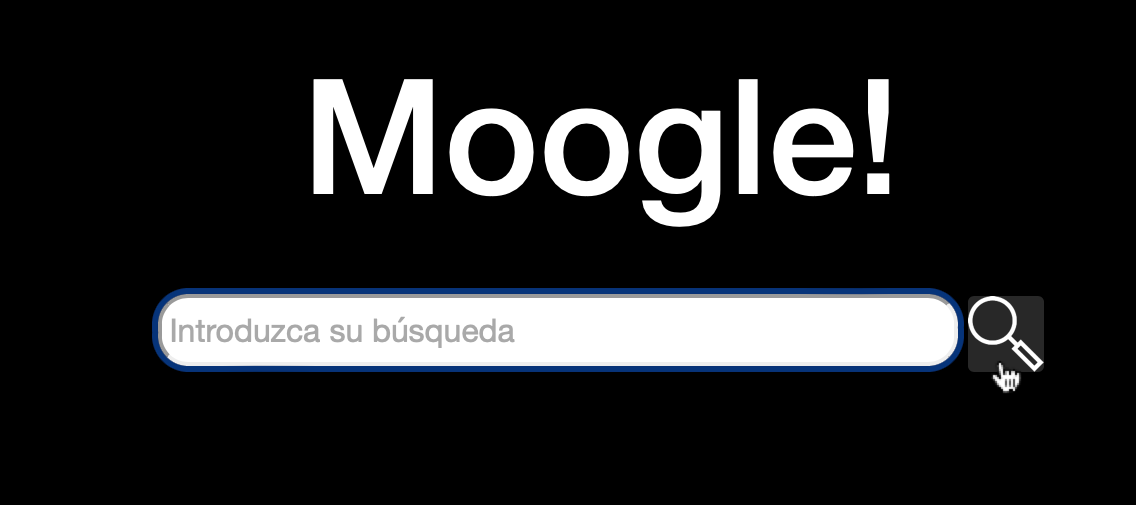
\includegraphics[scale=0.4]{Pictures/Buscando.png}\label{fig:Ejemplo de busqueda}
\end{center}
\begin{enumerate}
    \item Escribe tu búsqueda en el campo de entrada.
    \item Luego haz clic en el ícono de lupa o presiona la tecla ENTER para realizar la búsqueda.
\end{enumerate}
\newpage
\section{Funcionalidades extras de MOOGLE!}\label{sec:functions}

\subsection{Snippet}\label{sub:snippet}
El snippet muestra una porción del texto que contiene la primera aparición de la palabra de mayor
relevancia de su búsqueda.

\begin{center}
    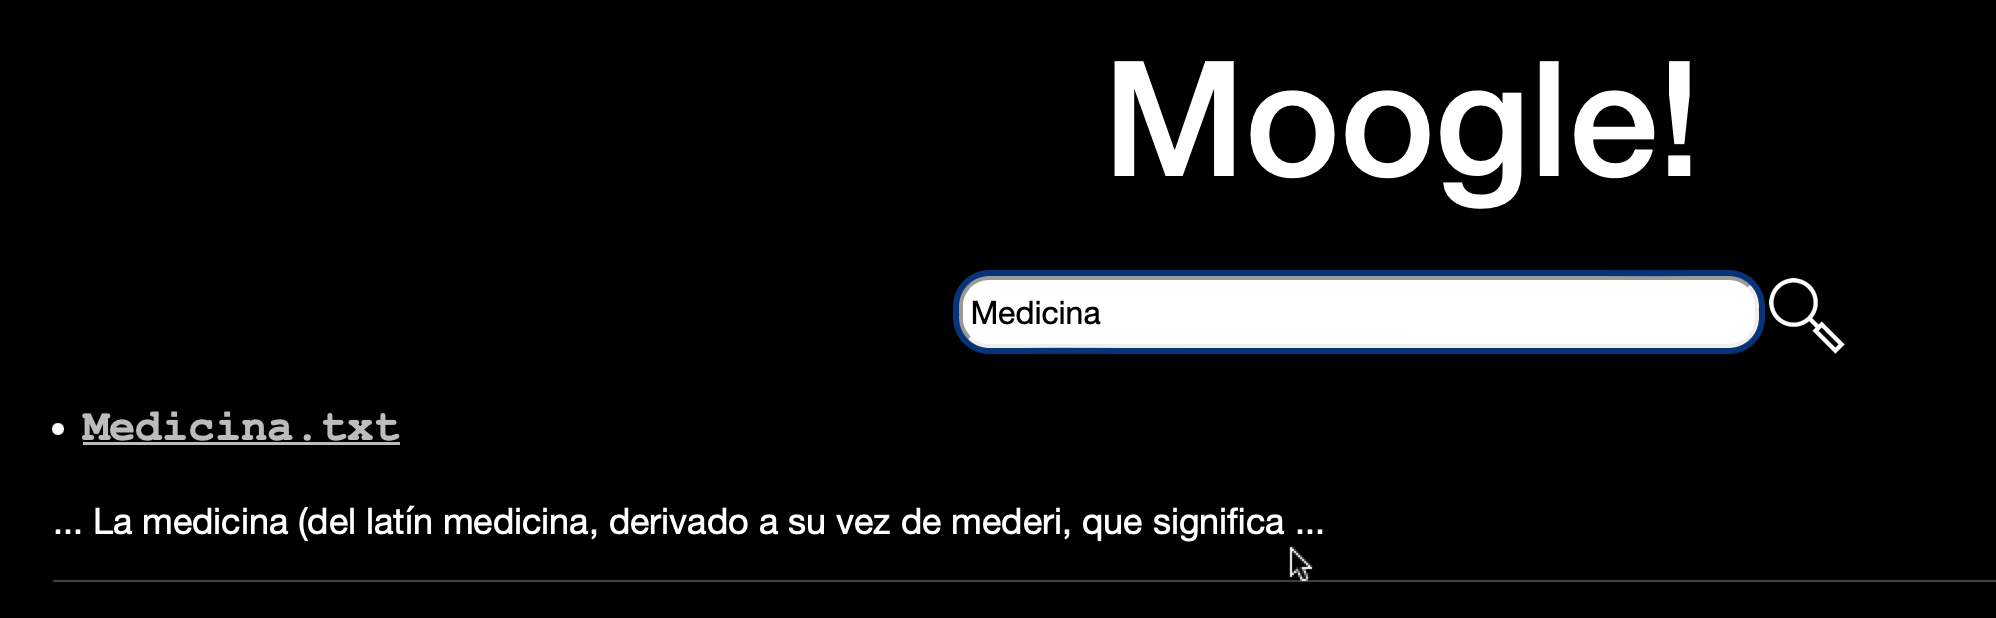
\includegraphics[scale=0.4]{Pictures/Snippet.png}
\end{center}


\subsection{Suggestion}\label{sub:suggestion}
Si al relaizar una búsqueda se equivoca en alguna palabra, MOOGLE! automáticamente te sugiere la palabra escrita correctamente 
o un remplazo lo más semejante posible. Por ejemplo si el usuario escribe Meddisina, no va a encontrar ningún resultado y va crear una sugerencia
indicando medicina.

\begin{center}
    
\includegraphics[scale=0.4]{Pictures/Suggestion.png}
\end{center}

\subsection{Abrir los documentos}\label{sub:OpenDocs}
Una vez realizada la búsqueda puedes abrir el documento desado simplemente haciendo clic en el nombre del documento.


\begin{center}
    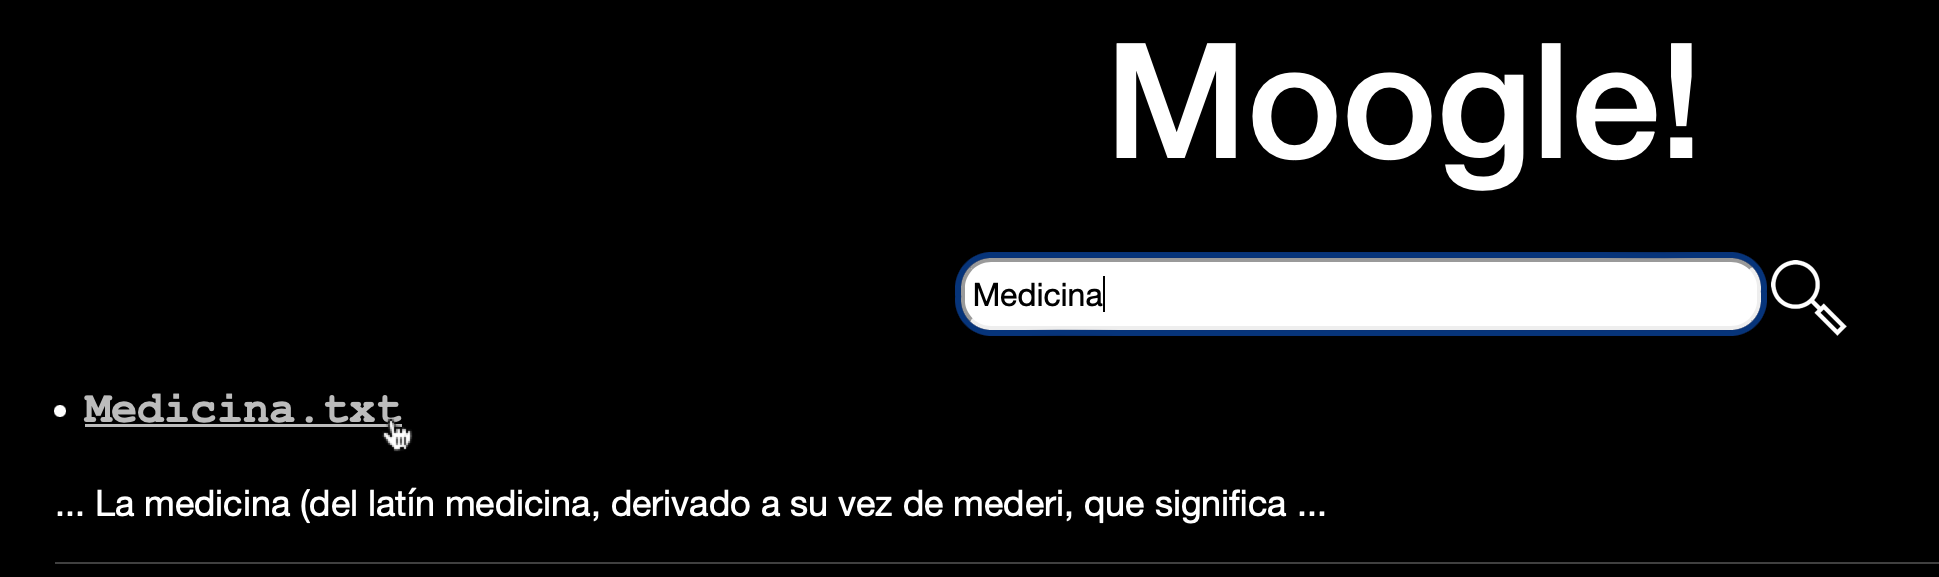
\includegraphics[scale=0.4]{Pictures/Opendocs.png}
\end{center}

\section{Utilidades del script proyecto.sh}

En el proyecto hay una carpeta llamada script que contiene un archivo llamado \texttt{proyecto.sh} , al ejecutarlo
posee un menú de opciones a realizar:

\begin{enumerate}
    \item run - Ejecutar el proyecto
    \item report - Compilar y generar informe del proyecto
    \item slides - Compilar y generar presentación del proyecto
    \item show-report - Ejecuta un programa para visualizar el informe del proyecto
    \item show-slides - Ejecuta un programa para visualizar la presentación del proyecto
    \item clean - Limpiar Ficheros innecesarios
\end{enumerate}

\end{document}